\documentclass{beamer}

\usepackage{amsmath}
\usepackage{float}
\usepackage{graphicx}

\usepackage{../cppenv}

\usepackage{../recdefs}

\usetheme{Bergen}
\usecolortheme{wolverine}

\title{CS100 Recitation 5}
\author{GKxx}
\date{March 21, 2022}

\AtBeginSubsection{
    \begin{frame}{Contents}
        \tableofcontents[currentsection, currentsubsection]
    \end{frame}
}

\begin{document}

\begin{frame}
    \maketitle
\end{frame}

\begin{frame}{Warmup}
    \begin{figure}[h]
        \centering
        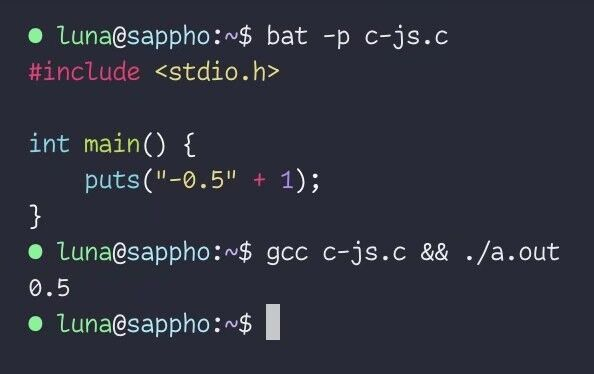
\includegraphics[width=\textwidth]{img/warmup_1.jpg}
    \end{figure}
\end{frame}

\begin{frame}{Warmup}
    \begin{figure}[h]
        \centering
        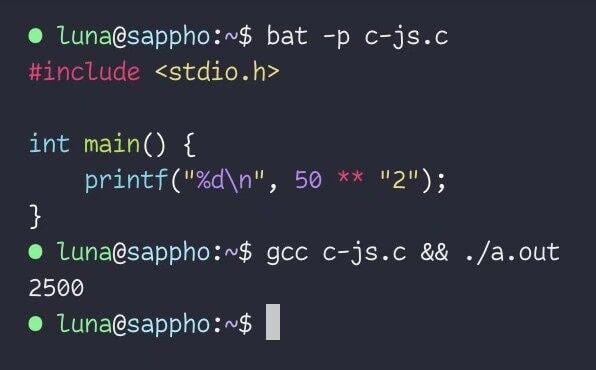
\includegraphics[width=\textwidth]{img/warmup_2.jpg}
    \end{figure}
\end{frame}

\section{IO}

\subsection{Streams}

\begin{frame}{Streams}
    \begin{dfn}[Stream]
        A \blue{stream} is a sequence of characters read from or written to an IO device.
    \end{dfn}
    The term \blue{stream} is intended to suggest that the characters are \blue{generated}, or \blue{consumed}, sequentially over time.\\
    \pause
    Standard input and output streams: \bluett{stdin} and \bluett{stdout}.
    \begin{itemize}
        \item \ttt{scanf}, \ttt{gets}, \ttt{getchar}: read from \ttt{stdin}.
        \item \ttt{printf}, \ttt{puts}, \ttt{putchar}: write to \ttt{stdout}.
    \end{itemize}
    By default, \ttt{stdin} and \ttt{stdout} are directed to the console.
\end{frame}

\subsection{Redirect to Files}

\begin{frame}{Redirection}
    We can redirect the standard streams to files:
    \begin{itemize}
        \item Use \ttt{< filename} to redirect \bluett{stdin} to a file.
        \item Use \ttt{> filename} to redirect \bluett{stdout} to a file.
        \pause
        \item Example: \ttt{./program < test.in > test.out}
        \item The online grader redirects your program and compares the output file with the answer file.
        \pause
        \item Input from any file terminates with \redtt{EOF}!
        \begin{itemize}
            \item \redtt{EOF} is a special character \teal{\#define}d as \ttt{-1}.
            \item It is suggested to use \bluett{int} to store the return-value of \ttt{getchar}, why?
        \end{itemize}
    \end{itemize}
\end{frame}

\begin{frame}[fragile]{Redirection}
    Use \ttt{freopen} to redirect:
    \begin{cpp}
int main() {
  freopen("in_file.txt", "r", stdin);
  freopen("out_file.txt", "w", stdout);
  // ...
}
    \end{cpp}
    \pause
    \begin{itemize}
        \item \bluett{stdin} and \bluett{stdout} are redirected to \ttt{"input\_file.txt"} and \ttt{"output\_file.txt"} respectively.
        \item \ttt{"r"}: read; \ttt{"w"}: write;
        \item There are also some other open modes.
    \end{itemize}
\end{frame}

\subsection{File Input and Output}

\begin{frame}[fragile]{File IO Functions}
    \begin{cpp}
int main() {
  FILE *in = fopen("in_file.txt", "r");
  FILE *out = fopen("out_file.txt", "w");
  int a, b;
  fscanf(in, "%d%d", &a, &b);
  fprintf(out, "%d\n", a + b);
  printf("%d\n", a + b);
  fclose(in);
  fclose(out);
  return 0;
}
    \end{cpp}
    \begin{itemize}
        \item \ttt{FILE}: a special type storing the information of a file.
        \item \ttt{fscanf}, \ttt{fprintf}, \ttt{fgets}, \ttt{fputs}, \ttt{fgetc}, \ttt{fputc}.
        \item Use \ttt{fopen} and \ttt{fclose}.
    \end{itemize}
\end{frame}

\subsection{String as a Stream}

\begin{frame}[fragile]{String IO Functions}
    \begin{itemize}
        \item \ttt{sscanf}: read data in an ``\ttt{scanf}-way'' from a string.
        \item \ttt{sprintf}: write data in a ``\ttt{printf}-way'' to a string.
    \end{itemize}
    \begin{cpp}
// roundabout way, just for demostration
int main() {
  char str[100];
  gets(str);
  int a, b;
  sscanf(str, "%d%d", &a, &b);
  char result[100];
  sprintf(result, "%d", a + b);
  puts(result);
  return 0;
}
    \end{cpp}
\end{frame}

\section{Structures}

\subsection{Define a Structure}

\begin{frame}[fragile]{Define a \bluett{struct}}
    \begin{cpp}
struct Tile {
  int num;
  char kind;
};
    \end{cpp}
    \pause
    \begin{itemize}
        \item A structure is a user-defined data type: \bluett{struct }\ttt{Tile}.
        \item We can define a variable of such type:
        \begin{cpp}
struct Tile t;
        \end{cpp}
        \pause
        \item Use \blue{member-access operator}:
        \begin{cpp}
t.num = 1;
t.kind = 's';
printf("%d\n", t.num);
        \end{cpp}
    \end{itemize}
\end{frame}

\begin{frame}[fragile]{Define a \bluett{struct}}
    An unnamed structure (which cannot be used after definition):
    \begin{cpp}
struct {
  int num;
  char kind;
};
    \end{cpp}
    \pause
    Defining both a structure and a variable (\textbf{not suggested coding-style}):
    \begin{cpp}
struct Tile {
  int num;
  char kind;
} t;
    \end{cpp}
\end{frame}

\begin{frame}[fragile]{Use \bluett{typedef}}
    \begin{cpp}
typedef long long LL;
    \end{cpp}
    Use \bluett{typedef}, so that we don't need the \bluett{struct} keyword everytime we use it.
    \begin{cpp}
typedef struct {
  int num;
  char type;
} Tile;
    \end{cpp}
\end{frame}

\begin{frame}[fragile]{Use \bluett{typedef}}
    Within the \bluett{typedef} declaration, you cannot refer to the type alia.
    \begin{cpp}
typedef struct {
  int value;
  Node *next;   // Error
} Node;
    \end{cpp}
    \pause
    Correct way: Give it a name first.
    \begin{cpp}
typedef struct _node_ {
  int value;
  struct _node_ *next;
} Node;
    \end{cpp}
\end{frame}

\begin{frame}[fragile]{Incomplete Type}
    You cannot define a member of the type itself:
    \begin{cpp}
struct Widget {
  struct Widget w;
  int x;
};
    \end{cpp}
    \begin{itemize}
        \item In syntax: during the definition, the type `\bluett{struct }\ttt{Widget}' is an \red{incomplete type}. It is not allowed to define a variable of an incomplete type.
        \item In semantics: What's the size of a `\bluett{struct }\ttt{Widget}'?
    \end{itemize}
\end{frame}

\begin{frame}[fragile]{Memory Alignment}
    \begin{cpp}
typedef struct {
  int num;
  char kind;
} Tile;
    \end{cpp}
    \bluett{sizeof}\ttt{(Tile) != }\bluett{sizeof}\ttt{(int) + }\bluett{sizeof}\ttt{(char)}
    \begin{itemize}
        \item In most implementations, the structure above takes 8 bytes. The storage will be aligned to multiple of 4.
    \end{itemize}
\end{frame}

\subsection{Operations on \bluett{struct}}

\begin{frame}[fragile]{Initialization}
    \begin{itemize}
        \item \blue{Default initialization} of a structure initializes every member by default (with an undefined value).
        \item \blue{Value initialization} of a structure initializes every member by value-initialization (with all types of `0').
        \pause
        \item \red{Copy initialization}: \ttt{Tile a = b;} copies the value of each member of \ttt{b} to \ttt{a}.
        \begin{itemize}
            \item \ttt{b} must be of type \ttt{Tile}.
        \end{itemize}
    \end{itemize}
\end{frame}

\begin{frame}[fragile]{Copy-assignment}
    \begin{cpp}
Tile a, b;
a.num = 1; a.kind = 's';
b = a;
    \end{cpp}
    The \blue{assignment operator} is generated by the compiler, which copies the value of each member of RHS to LHS.
\end{frame}

\begin{frame}[fragile]{A Unique Type}
    Every structure is a unique type.
    \pause
    \begin{cpp}
typedef struct {
  int num;
  char kind;
} Fake_tile;
Fake_tile ft;
ft = a;             // Error
Fake_tile ft2 = a;  // Error
    \end{cpp}
    \ttt{Fake\_tile} and \ttt{Tile} are \red{different types}, even though their definitions look the same.
\end{frame}

\begin{frame}[fragile]{Parameter and Return-value}
    \begin{cpp}
Tile next_tile(Tile t) {
  Tile next;
  next.num = t.num + 1;
  next.kind = t.kind;
  return next;
}
    \end{cpp}
    \pause
    \begin{itemize}
        \item When passing as an argument, it is in fact \textbf{copy-initializing} the parameter \ttt{Tile t}.
        \item When \ttt{return}ing from a function, it is in fact \textbf{copy-initializing} the temporary object generated by the calling expression. \red{(In C, and before C++11)}
    \end{itemize}
\end{frame}

\begin{frame}[fragile]{Parameter and Return-value}
    How many copies are there?
    \begin{cpp}
Tile next_tile(Tile t) {
  Tile next = t;
  ++next.num;
  return next;
}
int main() {
  Tile tile, tile2;
  tile.num = 1;
  tile.kind = 's';
  tile2 = next_tile(tile);
  return 0;
}
    \end{cpp}
\end{frame}

\begin{frame}[fragile]{Parameter and Return-value}
    \begin{cpp}
Tile next_tile(Tile t) {
  Tile next = t;
  ++next.num;
  return next;
}
// in main
Tile tile, tile2;
tile.num = 1; tile.kind = 's';
tile2 = next_tile(tile);
    \end{cpp}
    \begin{itemize}
        \item copy-initialization of parameter \ttt{t}.
        \item copy-initialization of \ttt{next};
        \item copy-initialization of a temporary object generated by \ttt{next\_tile(tile)}, with the value \bluett{return}ed.
        \item copy-assignment to \ttt{tile2}.
    \end{itemize}
\end{frame}

\begin{frame}[fragile]{Minor Optimization}
    Since \ttt{t} is a copy of the argument, we don't need another copy.
    \begin{cpp}
Tile next_tile(Tile t) {
  ++t.num;
  return t;
}
    \end{cpp}
    \pause
    \begin{itemize}
        \item \ttt{t} is destroyed immediately the function \bluett{return}s.
        \pause
        \item Why do we have to copy something \textbf{almost dead}, instead of simply \textbf{extending} its lifetime?
        \pause
        \item \red{C++11} solves this problem.
    \end{itemize}
\end{frame}

\begin{frame}[fragile]{Dynamic Allocation}
    \ttt{malloc} and \ttt{free} as usual.
    \begin{cpp}
Tile *thetile
  = (Tile *)malloc(sizeof(Tile));
Tile *manytiles
  = (Tile *)malloc(sizeof(Tile) * n);
free(thetile); free(manytiles);
    \end{cpp}
    \pause
    Access through pointers: dereference, and then access.
    \begin{cpp}
*thetile.num = 1;   // Error!
(*thetile).num = 1; // Correct
thetile->num = 1;   // Preferred
    \end{cpp}
    \begin{rmk}
        The \blue{member-access operator} has \textbf{higher} precedence than the \blue{dereference operator}.
    \end{rmk}
\end{frame}

\section{Coding}

\subsection{Good Coding-style}

\begin{frame}{Good Coding-style}
    \begin{itemize}
        \item The simpler, the better.
        \item Code in a modern way.
        \item Strive to compile warning-free at the maximum warning level.
        \item At least understand every warning completely.
        \item Read masterpieces, and imitate.
    \end{itemize}
\end{frame}

\subsection{Examples}

\end{document}